%%%%%%%%%%%%%%%%%%%%%%%%%%%%%%%%%%%%%%%%%%%%%%%%%%%%%%%%%%%%%%%%%%%%%%
% Dual Trace Communication Event Analysis
% 
% Author: Nora Huang
% Date: July 2017
% 
%%%%%%%%%%%%%%%%%%%%%%%%%%%%%%%%%%%%%%%%%%%%%%%%%%%%%%%%%%%%%%%%%%%%%%

\documentclass[paper=a4, fontsize=11pt]{scrartcl}
\usepackage[T1]{fontenc}
\usepackage{fourier}
\usepackage{tabu}
\usepackage{float}
\usepackage{afterpage}
\usepackage{booktabs}

\usepackage{longtable}
\usepackage{multicol}
\usepackage{multirow}

\usepackage[english]{babel}															% English language/hyphenation
\usepackage[protrusion=true,expansion=true]{microtype}	
\usepackage{amsmath,amsfonts,amsthm} % Math packages
\usepackage[pdftex]{graphicx}	
\usepackage{url}
\usepackage{listings}
\lstset{
    frame=single,
    breaklines=true
}


%%% Custom sectioning
\usepackage{sectsty}
\allsectionsfont{\centering \normalfont\scshape}


%%% Custom headers/footers (fancyhdr package)
\usepackage{fancyhdr}
\pagestyle{fancyplain}
\fancyhead{}											% No page header
\fancyfoot[L]{}											% Empty 
\fancyfoot[C]{}											% Empty
\fancyfoot[R]{\thepage}									% Pagenumbering
\renewcommand{\headrulewidth}{0pt}			% Remove header underlines
\renewcommand{\footrulewidth}{0pt}				% Remove footer underlines
\setlength{\headheight}{13.6pt}


%%% Equation and float numbering
\numberwithin{equation}{section}		% Equationnumbering: section.eq#
\numberwithin{figure}{section}			% Figurenumbering: section.fig#
\numberwithin{table}{section}				% Tablenumbering: section.tab#


%%% Maketitle metadata
\newcommand{\horrule}[1]{\rule{\linewidth}{#1}} 	% Horizontal rule

\title{
		%\vspace{-1in} 	
		\usefont{OT1}{bch}{b}{n}
		\normalfont \normalsize \textsc{Department of Computer Science,  University of Victoria} \\ [25pt]
		\horrule{0.5pt} \\[0.4cm]
		\huge Dual Trace Communication Event Analysis  \\
		\horrule{2pt} \\[0.5cm]
}
\author{
		\normalfont 								\normalsize
        Nora Huang\\[-3pt]		\normalsize
        \today
}
\date{}


%%% Begin document
\begin{document}
\maketitle

\section{Introduction}
Many network application vulnerabilities occur not just in one application, but in how they interact with other systems. These kinds of vulnerabilities can be difficult to analyze. Dual-trace analysis is one approach that helps the security engineers to detect the vulnerabilities in the interactive software. A dual-trace consist of two execution traces that are generated from two interacting applications. Each of these traces contains information including CPU instructions, register and memory changes of the running application. Communication information of the interacting applications is captured as the register or memory changes on their respective sides. Our research focuses on building a model to visualize and analyze dual-trace which would be available for various kinds of communication Type.

\section{Problem}
The major problem we are considering in dual-trace analysis is locating the synchronization point of the traces from both sides. We narrow down the problem into finding the sending points and receiving points of the communication messages and pair them. To do that in assembly level trace, there are three essential information to figure out: the messaging channel matching, individual message matching in each channel.

\section{Communication Types}
In order to synchronize the messaging of both side of the traces, we need to investigate the communication methods to figure out how they looks like in the assembly level traces.
There are so many communication methods exists in the real world. We are not covering all of them at a time, but start from narrowing down our study into some sort of communication methods. We start from investigating the messaging methods in Windows Communication Framework. There are two kinds of messaging channels in this framework, transport channels and protocol channel. We are current focus on transport channels. Transport channels read and write messages from the network (or some other communication point with the outside world). Example of transport channels are named pipes, MSMQ, HTTP and TCP channels. If our research turns out to be work in that particular communication methods, it is possible to extend it for more general use cases.
\subsubsection{Assembly Calling Convention}
Before we jump into each communication method, it is important to know some basic assembly calling convention.
Calling Convention is different for operating system and the programming language. Since we are looking into the messaging methods being used in windows communication framework, and since our case study in running on a Microsoft* x64 system, we only list Windows calling convention for the Microsoft* x64 calling convention, the additional register space let fastcall be the only calling convention (under x86 there were many: stdcall, thiscall, fastcall, cdecl, etc.). The rules for interfacing with C/C++ style functions:\par
\begin{enumerate}  
\item RCX, RDX, R8, R9 are used for integer and pointer arguments in that order left to right.
\item XMM0, 1, 2, and 3 are used for floating point arguments.
\item Additional arguments are pushed on the stack left to right. \ldots 
\item Parameters less than 64 bits long are not zero extended; the high bits contain garbage.
\item Integer return values (similar to x86) are returned in RAX if 64 bits or less.
\item Floating point return values are returned in XMM0.
\item Larger return values (structs) have space allocated on the stack by the caller, and RCX then contains a pointer to the return space when the callee is called. Register usage for integer parameters is then pushed one to the right. RAX returns this address to the caller.
\end{enumerate}

\subsection{Named pipes Channel}
A named pipe is a named, one-way or duplex pipe for communication between the pipe server and one or more pipe clients. All instances of the named pipe share the same pipe name, but each instance has it own buffers and handles. In here we only consider one to one server/client pairs. One server to multiple client scenario can always be divided into multiple server/client pairs cases.
\subsection{Related functions}
There are several system functions related to this communication type. However, only some of them are interested in our message matching mechanism since. They are list in Table\ref{namedpipefunctions}
\begin{table}
        \centering
        \caption{Named pipes system functions}
        \label{namedpipefunctions}
        \begin{tabular}{|l|l|l|l|l|l|l|}
            \hline
             \multirow{2}{*}{} &
               \multicolumn{2}{c|}{Channel Create functions} &
               \multicolumn{2}{c|}{message send functions} &
               \multicolumn{2}{c|}{message receive functions} \\
             \cline{2-7}
              & Function& Parameters & Function & Parameters  & Function & Parameters\\
             \hline
             Sever& CreateNamedPipe&  RCX: File handler & ReadFile &  RCX: File handler &WriteFile&\\
             \cline{3-3} \cline{5-5} \cline{7-7}
             &&RDX: Buffer Address&& RDX: Buffer Address &&\\
              \cline{3-3} \cline{5-5} \cline{7-7}
               &&R8:message length&&R8:message length &&\\
                \cline{1-3} \cline{5-5} \cline{7-7}
             Client & CreateFile & RCX: socket & & RCX: socke  &&\\
              \cline{3-3} \cline{5-5} \cline{7-7}
             &&RDX: Buffer Address&&RDX:Buffer Address&&\\
              \cline{3-3} \cline{5-5} \cline{7-7}
               &&R8: message length&&R8: message length&&\\
            \hline
        \end{tabular}
    \end{table}
\subsubsection{Blocking I/O}
\subsubsection{Non-Blocking I/O}
\subsection{MSMQ Channel}
\subsubsection{Blocking I/O}
\subsubsection{Non-Blocking I/O}
\subsection{HTTP Channel}
\subsection{TCP Channel}


\section{Prototype Building}
In this section we discuss the design of the prototype on how we match the send and receive events in the sender side trace and the receiver side trace. This prototype consist of three main components: defining the communication type, locating the communication events by matching the send and receive events on sender and receiver sides, navigating the located events in the sender and receiver traces. We provide the background information of the design of each component as well as its detail design in each corresponding subsection.
\subsection{User Defined Communication Type}
In our design, we don't specify any predefined communication type but give the user capacity to do that. By the user interface implemented in our tool, the user can defined their own communication type. This give the flexibility to the user to define what they are looking for. Each communication type consist of 4 system function calls. They are sender and receiver channel create/open, sender's send message function and receiver's receive message function. By indicating these the channel create/open function in both sender and receiver sides, the tool can acquire the channel's identifiers when they are created or opened. Later on the tool can match the send and received messages within a specific channel. The send and receive are used to located the event happened in the traces. The messages send and received are reconstructed from the memory state when the send and receive functions are called and returned. This detail of the match algorithm will be discuss later.

\subsubsection{Function Calls in the Traces}
The called functions' name can be inspected  by  search of the symbolic name in the executable binary or any DLLs which used by the program at the time when it is traced. This functionality exists in the current Atlantis. By importing the Dlls and execution  executable binary, Atlantis can list all called functions for the users in the Functions view. From this list, users can chose the interested functions and generate their interested communication type. In Figure\ref{functionsview} there is  an action item call "Add to Communication type" in the right click menu of the function entry. Figure \ref{dialog} shows the dialogue for entering the information for the added function. The needed information is the communication type's name. User can get the existing communication type list in the drop down menu. They can choose to add the current function to an exist communication type or they can add it to a new communication type by entering a new name. For the channel create/open function, the register holding the address of channel's name as input and the register holding the handle identification of the channel as output are required. For the send/receive function, the register holding the address of the send/receiver buffer, the register holding the length of the sending/receiving message and the register holding the channel's identification are required. As there are 4 functions for each communication type the user has to repeat this add function to communication type action for 4 time to generate one communication type.

\begin{figure}[h]
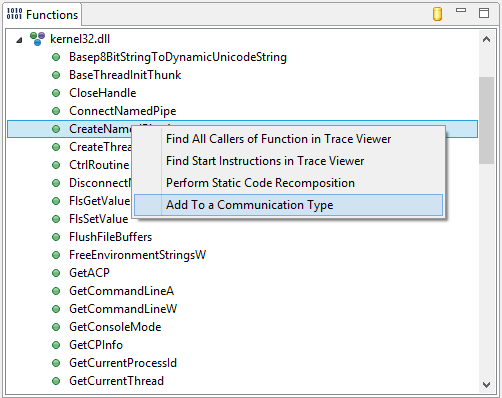
\includegraphics{functionsview}
 \caption{Add function to a Communication type from Functions View}
\label{functionsview}
\end{figure}

\begin{figure}[h]
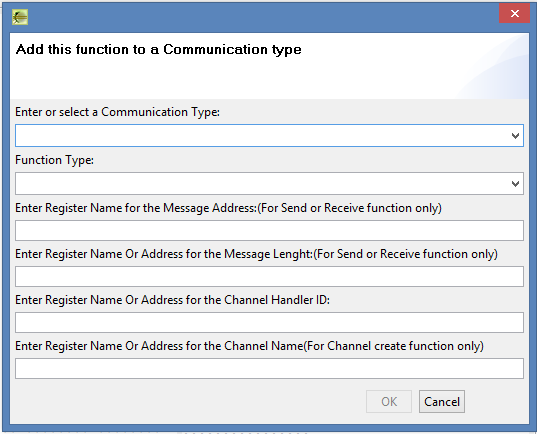
\includegraphics{dialog}
 \caption{Dialog to input information for a function adding to a communication type}
\label{dialog}
\end{figure}

\subsubsection{Communication Type Data Structure}
The defined communication type will be stored in a xml file. The list below shows the data structure of one communication type. 
\begin{lstlisting}
<messageTypesData>
    <parentFolder>.tmp</parentFolder>
    <messageTypes>
        <messageType>
            <name>namedPipe_clientsend</name>
            <sendFunction>
                <associatedFileName>Client</associatedFileName>
                <name>WriteFile</name>
                <messageAddress>RDX</messageAddress>
                <messageLengthAddress>R8</messageLengthAddress>
                <channelIdReg>RCX</channelIdReg>
            </sendFunction>
            <receiveFunction>
                <associatedFileName>Server</associatedFileName>
                <name>ReadFile</name>
                <messageAddress>RDX</messageAddress>
                <messageLengthAddress>R8</messageLengthAddress>
                <channelIdReg>RCX</channelIdReg>
            </receiveFunction>
            <sendChannelCreateFunction>
                <associatedFileName>Client</associatedFileName>
                <name>CreateFileA</name>
                <channelIdReg>RAX</channelIdReg>
                <channelNameAddress>RCX</channelNameAddress>
            </sendChannelCreateFunction>
            <receiveChannelCreateFunction>
                <associatedFileName>Server</associatedFileName>
                <name>CreateNamedPipeA</name>
                <channelIdReg>RAX</channelIdReg>
                <channelNameAddress>RCX</channelNameAddress>
            </receiveChannelCreateFunction>
        </messageType>
    </messageTypes>
</messageTypesData>
\end{lstlisting}


\subsubsection{Communication Type View}
A new view named Communication Types view is for the user defined communication types. All user defined communication type are listed in this view  as shown in Figure \ref{CommunicationTypeview}. User can change the name of a communication type, remove an existing communication type or searching of the match message occurrences of selected communication type by selecting the selected action item in the right click menu of an communication type entry. The matched messages are listed in the sub window of the view. By clicking the entry of the search  result, user can navigate to it's sender or receiver's corresponding instruction line as shown in Figure\ref{searchresult}. Message content in the memory view will be shown as well.


\begin{figure}[h]
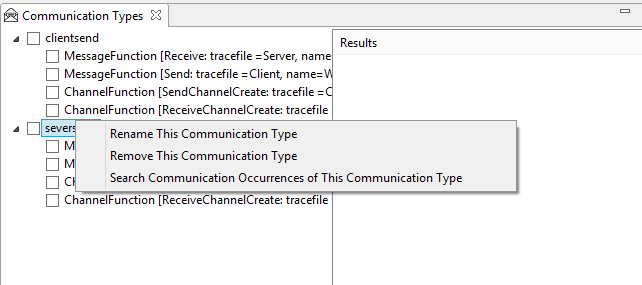
\includegraphics{CommunicationTypeview}
 \caption{New View: Communication Type View}
\label{CommunicationTypeview}
\end{figure}

\begin{figure}[h]
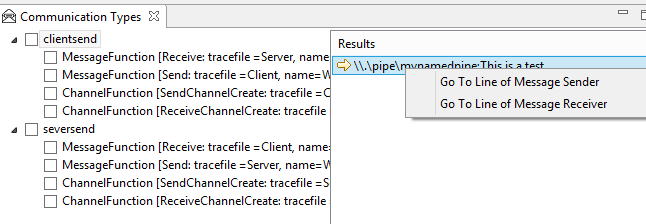
\includegraphics{searchresult}
 \caption{Right Click menu to navigate to send and receive event in the traces}
\label{searchresult}
\end{figure}

\subsection{Communication Event Searching}
The communication Event consists of the send message event in the sender side and receive message event in the receiver side. The communication event searching algorithm can be divided into three main steps: 1. search all channel create/open event in the sender and receiver side, save the handle id and corresponding channel name. 2. Search all message send and receive event in sender and receiver sides. 3. Matching the send/receive messages pair.
\subsubsection{Record opened Channel}

\subsubsection{Search send and receive Message}
\subsubsection{Matching the send/receive messages pair}
\subsubsection{Event Status: Success or Fail}
\subsubsection{Match Events Ordering}
\subsubsection{Matching Event Data Structure}
\begin{table}[h]
 \begin{center}
  \caption{Matched message pair data structure}
\label{table2}
\begin{tabular}{|c|c|c|c|c|}
      \hline
         Message& sender function name & sender line number  & receiver function name & receiver line number \\
       \hline
\end{tabular}
\end{center}
\end{table}
\subsection{Matching Event Visualization and Navigation}
\subsubsection{Navigating to The Sender/Receiver}
\subsubsection{Message Shown in memory view}


\section{Case Study}
Our prototype only be tested on traces of Microsoft 64 with C/C++ program. It seems too specific, however, the prototype can be adapted easily to other conventions. As long as users know the calling convention of their operating system, they can define their communication type with our tool. We list the related Microsoft 64 with C/C++ program convention here for reference and example. For more detail about the calling convention, users should refer to the operating system specification.\par
\subsubsection{communication type definition}

\subsection{Experiment Design}
\subsection{Result}
\subsection{Time Analysis}
\section{Limitation}


\section{Future Work}


\bibliographystyle{abbrv}
\bibliography{referencelist} 


%%% End document
\end{document}